\section{Experiment Results} \label{sec:exp_results}
Here, we present some preliminary findings. In order to explore the actual effects of \famsec{} on user behavior we designed a Mechanical Turk experiment where human users acted as dispatch supervisors of an autonomous vehicle (see Fig.~\ref{fig:experiment}). 

The responsibility of each participant was to decide whether the autonomous delivery vehicle should attempt to make a delivery, or decline the delivery. A successful attempt resulted in +1 point, failure in -1 point, and declining a delivery in -1/4 point. After being trained the participants saw a sequence of 43 different delivery scenarios with varying maps. Some preliminary data comparing the difference in cumulative `total score' is shown in Figure~\ref{fig:experiment}.

The total number of participants for this experiment was N=255, with n=\{63,63,64,65\} for conditions 0-3 respectively. In this situation Condition 0 is the control where participants didn't have self confidence metrics displayed. In Condition 1 the user was presented with \xQ{} only, they were presented with \xP{} only in Condition 2, and in Condition 3 users were presented with both \xQ{} and \xP{}.

\begin{figure}[tbp]
    \centering
    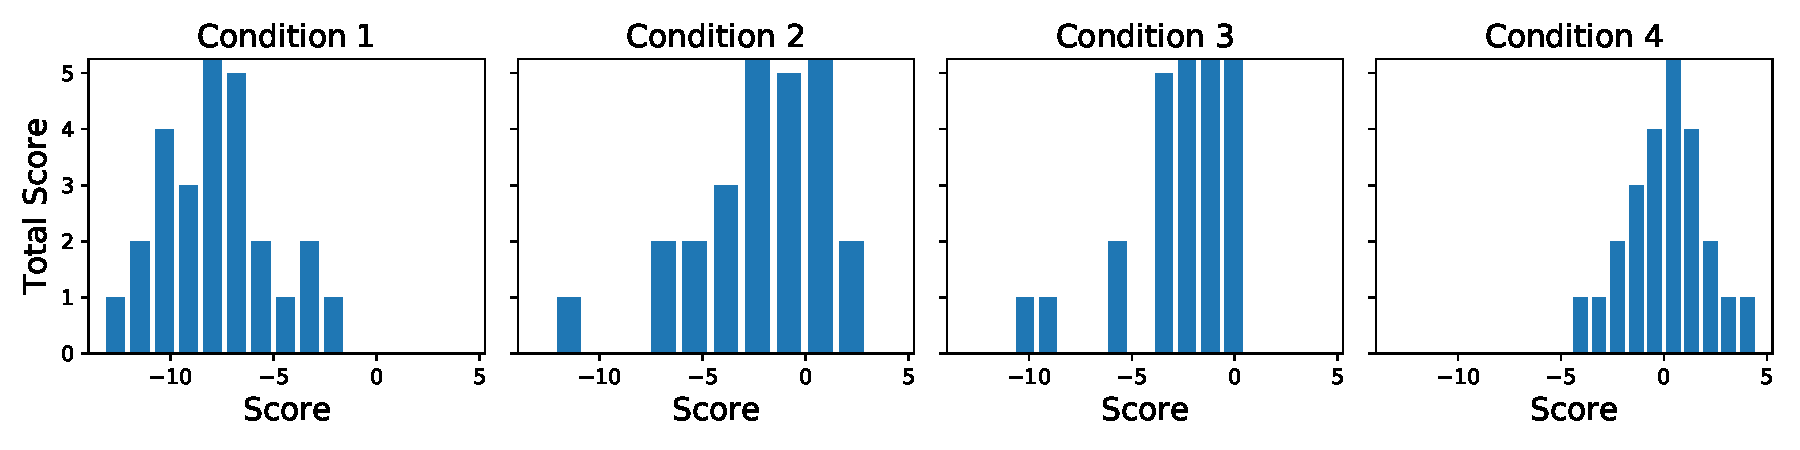
\includegraphics[width=1.0\linewidth]{Figures/test.pdf}
    \caption{Histogram of Scores From Each Condition}
    \label{fig:experiment}
\end{figure}

% \begin{table}[]
% \caption{Put in some statistics here---p-values}
% \label{tab:results}
% \begin{tabular}{lllll}
% \hline
% A & B & C & D \\ \cline{1-1}
% x\_Q(r=5.0) & 0.998 & 0.667 & 1.095 & 1.351 \\
% x\_Q(r=0.5) & 0.994 & 0.215 & 1.291 & 1.821 \\
% \end{tabular}
% \end{table}
